% Enable warnings about problematic code
\RequirePackage[l2tabu, orthodox]{nag}

\documentclass{resources/WeSTassignment}
\usepackage{tabularx}
\usepackage{booktabs}
\usepackage[utf8]{inputenc}
\usepackage{amsmath}
\usepackage{graphics}
\usepackage{graphicx}
\usepackage{changebar}
\usepackage{latexsym}
\usepackage{stmaryrd}
\usepackage{booktabs}
\usepackage{amsmath}
\usepackage{wasysym}
\usepackage[export]{adjustbox}
\usepackage[thinlines]{easytable}
\usepackage{framed}
\usepackage{color}
\usepackage{footnote}
\usepackage{listings}
\usepackage{framed}
\usepackage{tikz}
\usepackage[T1]{fontenc}
\usepackage{lmodern}

%\solutiontrue
% The lecture title, e.g. "Web Information Retrieval".
\lecture{Introduction to Web Science}
% The names of the lecturer and the instructor(s)
\author{%
  PD Dr. Matthias~Thimm\\{\normalsize\mailto{thimm@uni-koblenz.de}} \and
  Ipek Baris Schlicht\\{\normalsize\mailto{ibaris@uni-koblenz.de}} \and
  Kenneth Skiba\\{\normalsize\mailto{kennethskiba@uni-koblenz.de}}
}
% Assignment number.
\assignmentnumber{3}
% Institute of lecture.
\institute{%
  Institute of Web Science and Technologies\\%
  Department of Computer Science\\%
  University of Koblenz-Landau%
}
% Date until students should submit their solutions.
\datesubmission{01.12.2020, CEST 23:59}

% Specify bib file location.
\addbibresource{bibliography.bib}

\begin{document}

\maketitle

\centering \textbf{Team:} Bravo\\
\centering \textbf{Members:}\\
\centering  Gaurav Kumar (220200656)\\
\centering  Pavithree Shetty (220200661)\\
\centering  Nisha Sharma (220202359)\\

\section{Recursive Query: DNS \hfill{20 Points}}
For this task we will extend the routing table from the fourth task on Assignment 1.

In the following schema rectangles represent the networks, with there name inside. The circles are the routers. An edge between a router and a network means, that a router is part of this network and has the MAC address written at the edge in blue, while the interface is written in black.

In the routing table below you find an entry for every router. One entry in the routing table of a router contains a three tuple of Destination, Next Hop and Interface. 
\begin{figure}[h]
    \centering
    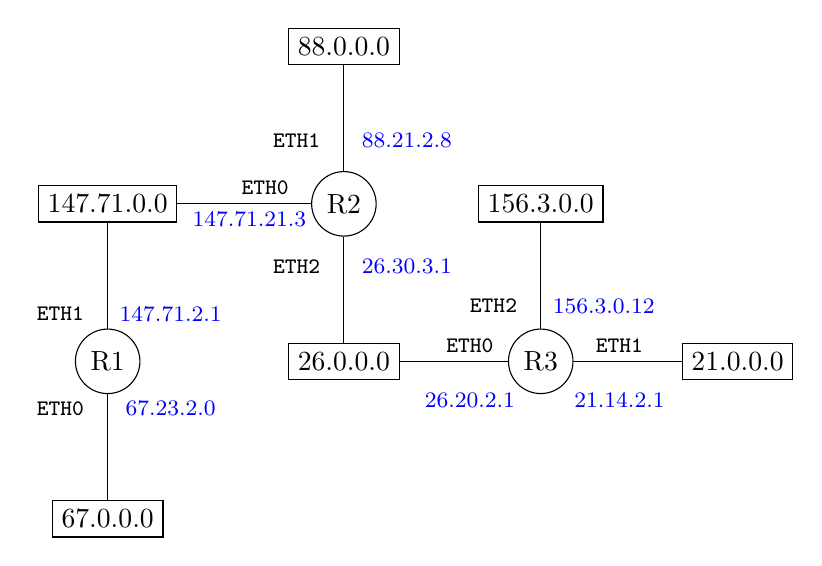
\begin{tikzpicture}
\node[draw, rectangle](C1) at (0,0) {67.0.0.0};
\node[draw, rectangle](C2) at (0,4) {147.71.0.0};
\node[draw, rectangle](C3) at (3,6) {88.0.0.0};
\node[draw, rectangle](C4) at (3,2) {26.0.0.0};
\node[draw, rectangle](C5) at (8,2) {21.0.0.0};
\node[draw, rectangle](C6) at (5.5,4) {156.3.0.0};

\node[draw, circle](R1) at (0,2) {R1};
\node[draw, circle](R2) at (3,4) {R2};
\node[draw, circle](R3) at (5.5,2) {R3};

\draw[-](C1) to (R1);
\node (R1_eth0) at (-0.6,1.4) {\texttt{\footnotesize{ETH0}}};
\node (R1_mac0) at (0.8,1.4) {\textcolor{blue}{\footnotesize{67.23.2.0}}};
\draw[-](R1) to (C2);
\node (R1_eth1) at (-0.6,2.6) {\texttt{\footnotesize{ETH1}}};
\node (R1_ma1) at (0.8,2.6) {\textcolor{blue}{\footnotesize{147.71.2.1}}};
\draw[-](C2) to (R2);
\node (R2_eth0) at (2,4.2) {\texttt{\footnotesize{ETH0}}};
\node (R2_mac0) at (1.8,3.8) {\textcolor{blue}{\footnotesize{147.71.21.3}}};
\draw[-](R2) to (C3);
\node (R2_eth1) at (2.4,4.8) {\texttt{\footnotesize{ETH1}}};
\node (R2_ma1) at (3.8,4.8) {\textcolor{blue}{\footnotesize{88.21.2.8}}};
\draw[-](R2) to (C4);
\node (R2_eth2) at (2.4,3.2) {\texttt{\footnotesize{ETH2}}};
\node (R2_ma2) at (3.8,3.2) {\textcolor{blue}{\footnotesize{26.30.3.1}}};
\draw[-](C4) to (R3);
\node (R3_eth0) at (4.6,2.2) {\texttt{\footnotesize{ETH0}}};
\node (R3_mac0) at (4.6,1.5) {\textcolor{blue}{\footnotesize{26.20.2.1}}};
\draw[-](R3) to (C5);
\node (R3_eth1) at (6.5,2.2) {\texttt{\footnotesize{ETH1}}};
\node (R3_mac1) at (6.5,1.5) {\textcolor{blue}{\footnotesize{21.14.2.1}}};
\draw[-](R3) to (C6);
\node (R3_eth2) at (4.9,2.7) {\texttt{\footnotesize{ETH2}}};
\node (R3_mac2) at (6.3,2.7) {\textcolor{blue}{\footnotesize{156.3.0.12}}};
\end{tikzpicture}
    \caption{Routing schematic representation}
    \label{fig:schematic_routing}
\end{figure}

\begin{table}[h]
    \centering
    \scalebox{0.8}{
\begin{tabular}{|l|l|l|l|l|l|l|l|l|}
\hline
\multicolumn{3}{|c|}{Router 1}        & \multicolumn{3}{c|}{Router 2}         & \multicolumn{3}{c|}{Router 3}        \\ \hline
Destination & Next Hop    & Interface & Destination & Next Hop    & Interface & Destination & Next Hop   & Interface \\ \hline
67.0.0.0    & 67.23.2.0   & eth0      & 147.71.0.0  & 147.71.21.3   & eth0      & 26.0.0.0  & 26.20.2.1 & eth0      \\ \hline
147.71.0.0    & 147.71.2.1   & eth1      & 88.0.0.0  & 88.21.2.8 & eth1      & 21.0.0.0   & 21.14.2.1  & eth1      \\ \hline
88.0.0.0  & 147.71.21.3 & eth1      & 26.0.0.0    & 26.30.2.1    & eth2      & 88.0.0.0    & 26.30.3.1 & eth0      \\ \hline
26.0.0.0    & 147.71.21.3 & eth1      & 67.0.0.0    & 147.71.2.1 & eth0      & 147.71.0.0  & 26.30.3.1  & eth0      \\ \hline
21.0.0.0  & 147.71.21.3   & eth1      & 21.0.0.0    & 26.20.2.1 & eth2      & 67.0.0.0    & 26.30.3.1  & eth0      \\ \hline
156.3.0.0  & 147.71.21.3   & eth1      & 156.3.0.0    & 26.20.2.1 & eth2      & 156.3.0.0    & 156.3.0.12  & eth2      \\ \hline
\end{tabular}
}
    \caption{Routing table}
    \label{sol:tab:routing_table}
\end{table}

Let us assume a client with the following IP address 67.4.5.2 wants to resolve the following domain  \texttt{subdomain.webscienceexample.com} using the DNS.

You can further assume the root name server has the IP address of 88.8.2.1 and the name-server for \texttt{com} has the IP address 156.3.20.2. 
Finally the domain is handled by a name server with the IP of 21.155.36.7.

Please explain how the traffic flows through the network in order to resolve the recursive DNS query. You can assume ARP tables are cached so that no ARP-requests have to be made.
\subsection{Solution:}
\begin{enumerate}
\item The client with IP address \textbf{67.4.5.2} reaches the router\textbf{R1} in order to issue a \textbf{DNS request} to the root name server with the destination IP address \textbf{88.8.2.1}. Now the router \textbf{R1} looks into its routing table and finds the next hop to be \textbf{147.71.2.3} in order to reach the network \textbf{88.0.0.0} and reaches the Router \textbf{R2} . Now since router \textbf{R2} is directly connected to the network \textbf{88.0.0.0},it delivers the \textbf{IP packet} requesting the IP address of \textbf{subdomain.webscienceexample.com} to the root name server at   \textbf{88.8.2.1} .
\item The root name server responds with the referral to top level domain \textbf{.com} with IP address \textbf{156.3.20.2}. Now this IP packet is routed back from the destination \textbf{88.8.2.1} to client at \textbf{67.4.5.2}. This packet from router \textbf{R2} reaches router \textbf{R1} with the next hop \textbf{147.71.2.1} . Since the network \textbf{67.0.0.0} is directly connected to router \textbf{R1}. The packet gets delivered to the client at \textbf{67.4.5.2}.
\item The client sends a another DNS request to the name server with IP \textbf{156.3.20.2}. This IP packet reaches router \textbf{R1}.The router repeats the process of looking into its table and routes the packet to router \textbf{R2} through next hop \textbf{147.71.21.3}. Now the router 2 looks into its table and routes the packet to router \textbf{R3} through next hop \textbf{26.20.2.1}.Router \textbf{R3} delivers the IP packet to the name server at destination \textbf{156.3.20.2}. 
\item The name server now responds with an IP packet consisting of the address of the name server \textbf{webscienceexample.com} to the client which is now acting as the destination at \textbf{67.4.5.2}. This packet is routed from \textbf{R3} to router \textbf{R2} with the hop \textbf{26.30.3.1}. The packet from router \textbf{R2} reaches router \textbf{R1} through next hop \textbf{147.71.2.1}.The router \textbf{R1} delivers the packet to the client.
\item Now the client sends the request to the name server \textbf{webscienceexample.com} at destination with IP \textbf{21.155.36.7}. This packet is routed from \textbf{R1} to \textbf{R2} through next hop \textbf{147.71.21.3}. The packet is routed from \textbf{R2} to \textbf{R3} through next hop \textbf{26.20.2.1}. The request is delivered to the name server through \textbf{R3}.
\item The name server sends an IP packet with requested information to the client at destination \textbf{67.4.5.2}. This packet is routed from \textbf{R3} to router \textbf{R2} with the hop \textbf{26.30.3.1}. The packet from router \textbf{R2} reaches router \textbf{R1} through next hop \textbf{147.71.2.1}.The router \textbf{R1} delivers the packet to the client.

\end{enumerate}

	
\section{Internet Architecture \hfill{20 Points}}
\begin{enumerate}
    \item Explain in your own words the four layer of the Internet architecture.
    \item Formulate an example to show the usage of the aforementioned layers.
\subsection{Four layers of the Internet Protocol suite:}
\begin{enumerate}
    \item \textbf{First Layer - Link Layer}
	\begin{itemize}
    		\item It is a protocol or group of methods that operate only on host's link.
		\item The link is the physical and logical network component used to interconnect hosts or nodes in the network.
		\item For example, how ethernet worked on a Local area network.
	\end{itemize}
    \item \textbf{Second Layer - Internet Layer}
	\begin{itemize}
    		\item It is a group of internetworking methods, protocols and specifications that are used to transport datagrams or packets from the originating host across network boundaries, if possible to the destination host specified by a network address or IP address.
		\item It derives its name from function of facilitating internetworking, connecting multiple networks with each other through gateways and routers.
	\end{itemize}
    \item \textbf{Third Layer - Transport Layer}
	\begin{itemize}
    		\item It provides end-to-end communication services for applications within a layered architecture of network components and protocols.
		\item It also provides convenient services such as connection-oriented data stream support, reliability, flow control, and multiplexing.
	\end{itemize}
    \item \textbf{Fourth Layer - Application Layer}
	\begin{itemize}
    		\item It is an abstraction layer reserved for process-to-process communications across an Internet Protocol computer network.
		\item It uses transport layer protocols to establish process-to-process connections via ports. For example, Domain Name System, Simple Mail Transfer Protocol, etc.
	\end{itemize}
	\bigbreak   REFERENCE: \url{https://commons.wikimedia.org/wiki/File:Data_Flow_of_the_Internet_Protocol_Suite.PNG}
\begin{figure}[h!]
  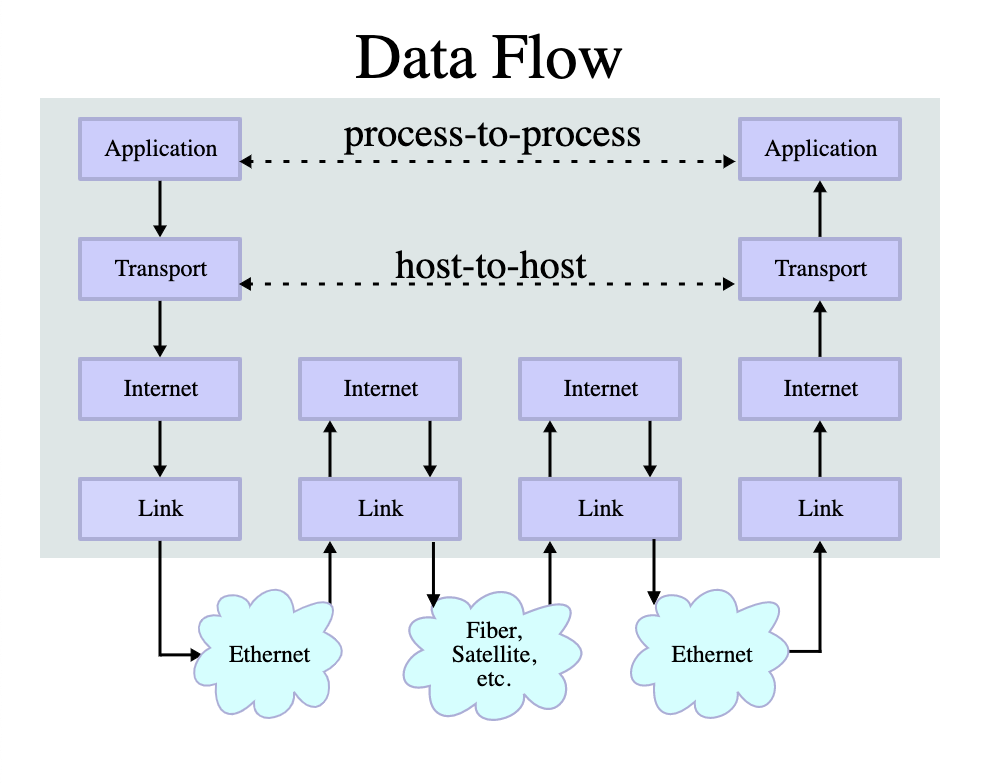
\includegraphics[width=\linewidth]{resources/data-flow.png}
  \caption{Data Flow in the four layers}
  \label{Data Flow of the Internet Protocol Suite}
\end{figure}
\end{enumerate}
\subsection{Example to show usage of the four layers:}
Let’s suppose we’re using Skype on a laptop. We’re messaging our friend, who’s using Skype on their phone from a different network.
\begin{itemize}
	\item Skype, as a network-connected application, uses \textbf{Layer 4 (Application)} protocols like Telnet. If we send our friend a picture of our cat, Skype would be using the File Transfer Protocol (FTP).
	\item \textbf{Layer 3 (Transport)} receives data from Layer 4 and segments it. Each segment, or data unit, has a source and destination port number, as well as a sequence number. The port number ensures that the segment reaches the correct application. The sequence number ensures that the segments arrive in the correct order.
	\item \textbf{Layer 2} (Internet) transmits data segments between networks in the form of packets. When we message our friend, this layer assigns source and destination IP addresses to the data segments. Our IP address is the source, and our friend’s is the destination. Layer 2 also determines the best paths for data delivery.
	\item \textbf{Layer 1 (Link)} receives packets from Layer 2. Whereas Layer 3 performs logical addressing (IPv4, IPv6), Layer 1 performs physical addressing. It adds sender and receiver MAC addresses to the data packet to form a data unit called a frame. Layer 1 enables frames to be transported via local media (e.g. copper wire, optical fiber, or air). This layer is embedded as software in our computer’s Network Interface Card (NIC). In short, Layer 1 allows the upper network layers to access media, and controls how data is placed and received from media.
\end{itemize}

\section{World Wide Web \hfill{14 Points}}
\subsection{Two different motivation points for the construction of the world wide web}
\begin{enumerate}
    \item \textbf{Decentralize Network}
	\begin{itemize}
    		\item Earlier every data was organized and transmitted through a centralised system.
		\item Slowed the process of transmission and information exchange between two host.
		\item Not everyone had the freedom to contribute for the development of this system.
		\item To give Power to people rather than only a central admistration.
	\end{itemize}
    \item \textbf{Exchange of information}
	\begin{itemize}
    		\item The major issue faced while data transmission was the exchange of information was very restricted due to various contraints.
		\item Both host was required to have same system which were compatible with each other for data transmission.
		\item Both host was required to have same operating system, software etc for successful data transmission.
		\item To create a network which is independent of any technical restriction
	\end{itemize}
    \item \textbf{Crossing network boundaries}
	\begin{itemize}
    		\item Another issue which movitate Tim Berners Lee to create was being able to connect to system beyond network boundaries.
		\item It was time consuming and required user to remember a lot of commands for transmission.
		\item To be able to reach people far away from the host.
	\end{itemize}
    \item \textbf{Combining Hypertext with network}
	\begin{itemize}
    		\item To be able to combine the capability of hypertext with transmission of data over the network.
	\end{itemize}
\end{enumerate}

\subsection{Five design principles of the world wide web}
\begin{enumerate}
    \item \textbf{Test of Independent invention}
	\begin{itemize}
    		\item In a centralized system if there are two similar ideas, one would be discared thereby lossing the efforts and idea
		\item World wide web gave the opportunity to those similar ideas to coexist by integrating them smoothly and imporve those idea with incremental efforts
	\end{itemize}
    \item \textbf{HyperText}
	\begin{itemize}
    		\item The Hypertext was combined with networking capability to create world wide web
	\end{itemize}
    \item \textbf{Networking Capability}
	\begin{itemize}
    		\item The ability to reach beyond the network boundaries.
	\end{itemize}
    \item \textbf{URL}
	\begin{itemize}
    		\item Global naming convention for every website which is easy to remember
		\item The URL need not be registered, only the domain names are required to register
	\end{itemize}
    \item \textbf{No single point of failure}
	\begin{itemize}
    		\item Any subdomain may no longer be available/down, however web as a whole will not stop working.
	\end{itemize}
    \item \textbf{Scaling}
	\begin{itemize}
    		\item World wide web has the capabiliy to scale as and when the number of host/users starts increasing.
	\end{itemize}
    \item \textbf{Simple Language}
	\begin{itemize}
    		\item It was developed using html which is very simple and minimum syntax to remember, which helps people contribute easily.
	\end{itemize}
    \item \textbf{Effortless}
	\begin{itemize}
    		\item Accessing and contributing was made effortless with around 80\% interaction and only 20\% efforts
	\end{itemize}
    \item \textbf{Easy to provide content using http}
    \item \textbf{Can work independently and contribute anonymously}
\end{enumerate}


\section{Python Programming \hfill{26 points}}
\subsection{URL Parser \hfill{13 points}\label{url_parser}}
Write a Python script called as \texttt{urlparser.py}. The script parses an url into the segments that are explained in the lecture \textbf{Internet vs WWW}, and additionally extracts top-level domains as one segment \footnote{https://en.wikipedia.org/wiki/Top-level\_domain}. When you execute the script (e.g \texttt{python -m urlparser https://west.uni-koblenz.de/studying/ws2021}) at the command-line, a dictionary containing the url and its segments should be returned. For the optional parts, you may use \texttt{None} values. 

Take a screenshot of the terminal output of your script for the following URLs
\begin{enumerate}
    \item \url{https://www.facebook.com/photo.php?fbid=2068026323275211&set=a.269104153167446&type=3&theater}
\begin{figure}[h!]
  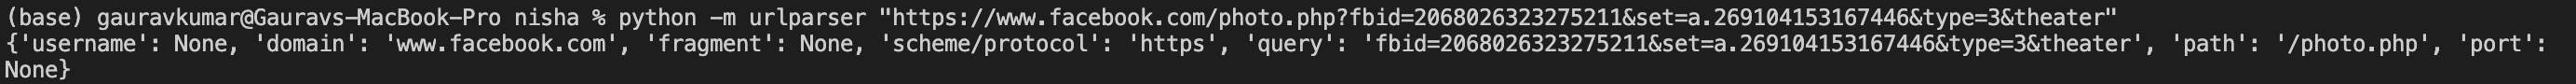
\includegraphics[width=\linewidth]{resources/facebook_urlparser.png}
  \caption{Screenshot of the url prsing}
  \label{Screenshot of the url parsing}
  \end{figure}
    \item \url{http://www.blog.google.uk:1000/path/to/myfile.html?key1=value1&key2=value2#InTheDocument}
\begin{figure}[h!]
  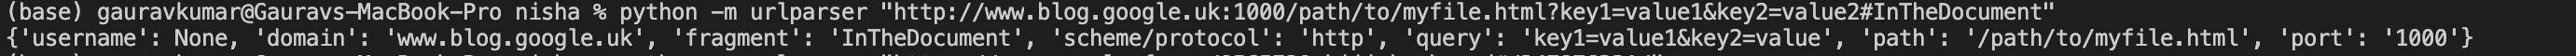
\includegraphics[width=\linewidth]{resources/blog_google_urlparser.png}
  \caption{Screenshot of the url prsing}
  \label{Screenshot of the url parsing}
  \end{figure}
    \item \url{https://www.overleaf.com/9565720ckjijuhzpbccsd#/347876331/}
    \begin{figure}[h!]
  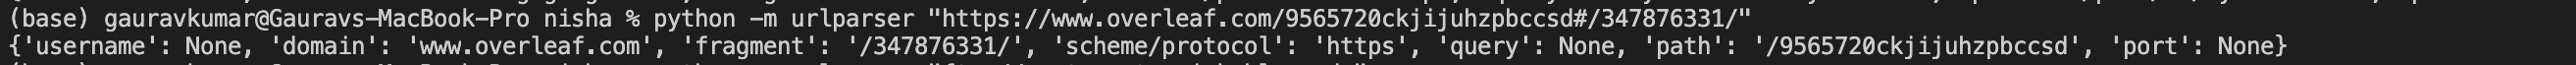
\includegraphics[width=\linewidth]{resources/overleaf_urlparser.png}
  \caption{Screenshot of the url prsing}
  \label{Screenshot of the url parsing}
  \end{figure}
    \item \url{ftp://root@west.uni.koblenz.de}
    \begin{figure}[h!]
  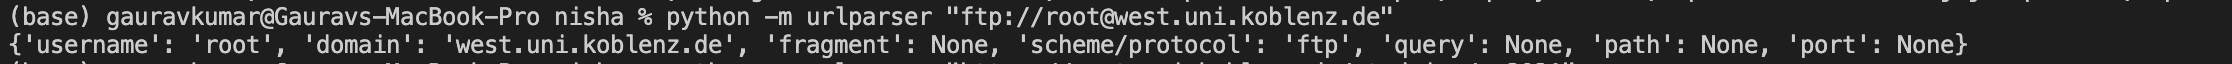
\includegraphics[width=\linewidth]{resources/root_urlparser.png}
  \caption{Screenshot of the url prsing}
  \label{Screenshot of the url parsing}
  \end{figure}
    \item \url{https://west.uni-koblenz.de/studying/ws2021}
    \begin{figure}[h!]
  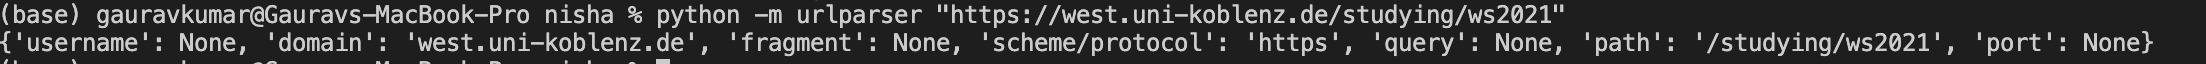
\includegraphics[width=\linewidth]{resources/unikoblenz_urlparser.png}
  \caption{Screenshot of the url prsing}
  \label{Screenshot of the url parsing}
  \end{figure}
    
\end{enumerate}

You are not allowed to use any specific libraries that help in url parsing and regular expressions. 

\subsection{Simple HTTP Web Client \hfill{13 points}}
\begin{figure}[h!]
  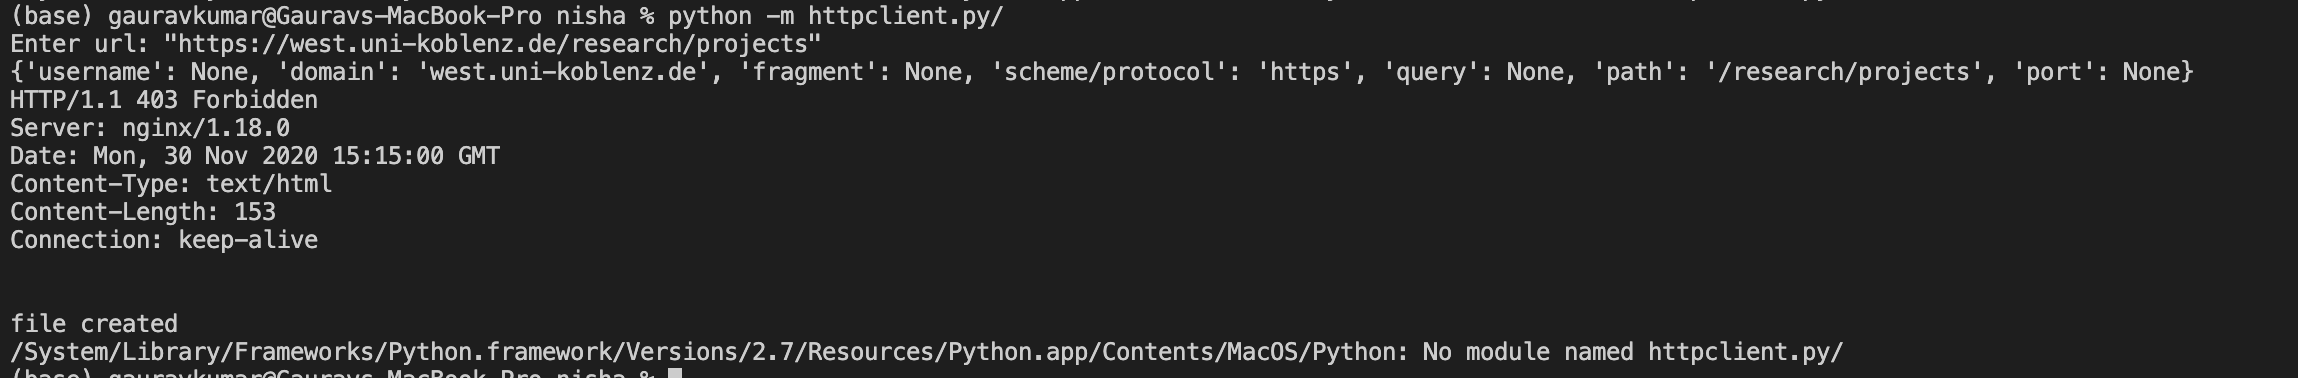
\includegraphics[width=\linewidth]{resources/403.png}
  \caption{403 status code}
  \label{403 status code}
\end{figure}
\begin{itemize}

\item For url \textbf{https://west.uni-koblenz.de/research/projects}, returned code \textbf{403}, since this domain is restricting to let any external source connect to it through the defailt socket without providing appropriate authentication.

\end{itemize}
\begin{figure}[h!]
  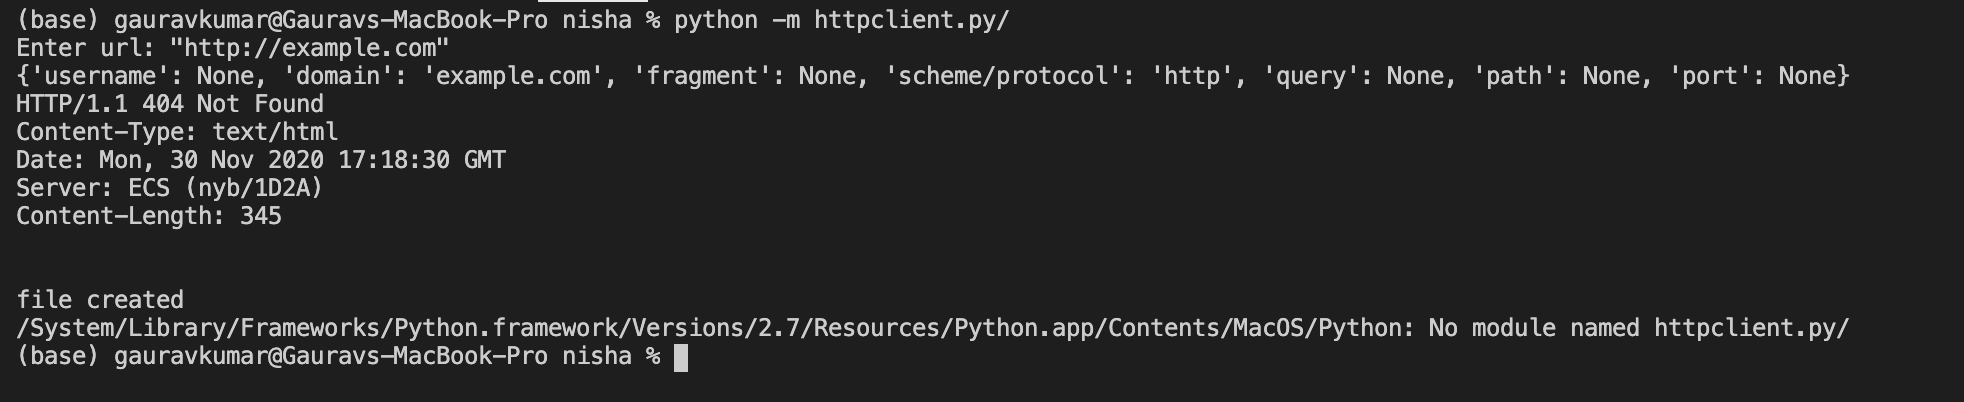
\includegraphics[width=\linewidth]{resources/404_a.png}
  \caption{301 status code}
  \label{301 status code}
\end{figure}
\begin{itemize}

\item For url \textbf{http://example.com}, returned code \textbf{404}, since this domain no longer exists or never existed.

\end{itemize}
\begin{figure}[h!]
  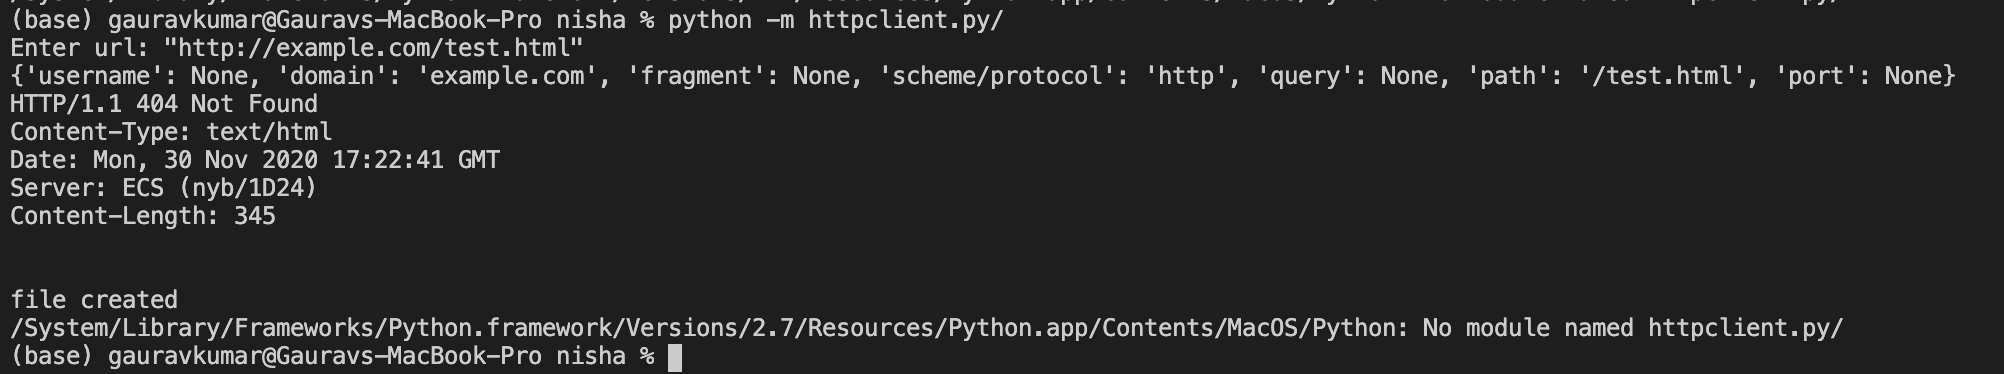
\includegraphics[width=\linewidth]{resources/404_b.png}
  \caption{404 status code}
  \label{404 status code}
\end{figure}
\begin{itemize}

\item For url \textbf{http://example.com/test.html}, returned code \textbf{404}, since this domain no longer exists or never existed.

\end{itemize}
    
\end{document}